\subsection{JAM based on Surface Brightness}

\subsubsection{... with "Mass-follows-Light" and Velocity Anisotropy}

[TO DO]

\begin{figure*}
\centering
\begin{minipage}{.5\textwidth}
  \centering
  \includegraphics[height=6cm]{fig/jam_A2_vrms.ps}
  \caption{??? Preliminary crappy caption: Failed try to fit a mass-follows-light model to the central regions of the galaxy. "Best fit" velocity anisotropy $\beta = -1/2$ is pegged at lower limit. ??? [TO DO: nice caption]}
  \label{fig:???}
\end{minipage}%
\begin{minipage}{.5\textwidth}
  \centering
  \includegraphics[height=6cm]{fig/lensing_JAM_comparision.ps}
  \caption{??? Preliminary crappy caption: Observed vrms is overplotted (not fitted) with best fit lens mass models for $\alpha = 1$ (red) and $\alpha = 1.1$ (green).??? [TO DO: nice caption]}
  \label{fig:???}
\end{minipage}
\end{figure*}

\subsubsection{... with Increasing Mass-to-Light Ratio Gradient}

[TO DO]

\begin{figure*}
\centering
\begin{subfigure}{.5\textwidth}
  \centering
  \includegraphics[height=6cm]{fig/jam_G_vrms.ps}
  \caption{???}
  \label{fig:???}
\end{subfigure}%
\begin{subfigure}{.5\textwidth}
  \centering
  \includegraphics[height=6cm]{fig/jam_G_enclMass.ps}
  \caption{???}
  \label{fig:???}
\end{subfigure}
\caption{??? Using the surface brightness MGE for the dynamical modelling: each Gaussian got it's own M/L such that the overall M/L is increasing with radius. This is the best fit model. The enclosed mass is overplotted with Einstein mass with 4\% error (overplotted, not fitted). ??? [TO DO: nice caption]}
\label{fig:???}
\end{figure*}

\subsubsection{... with the Lens Mass Model}

[TO DO]
